\section{INGENIERÍA DEL SISTEMA}

\subsection{Descripción general de la solución}

La solución implementada corresponde a un buscador semántico de alojamientos temporales
construido sobre una ontología OWL/RDF cargada en Apache Jena Fuseki. La interfaz web
permite realizar búsquedas en lenguaje natural, interpretar criterios estructurados y
presentar resultados en tres idiomas. La arquitectura fue pensada para que la ontología
sea el núcleo del sistema y no un artefacto secundario: tanto la recuperación de
resultados como la internacionalización dependen directamente del grafo semántico.

Desde el punto de vista de ejecución, el sistema combina tres componentes principales:
una base de conocimiento ontológica, un \textit{triple store} con endpoint SPARQL y una
aplicación web que consume ese endpoint. El enriquecimiento con DBpedia se integra en la
propia ontología mediante alineaciones y enlaces semánticos, lo que permite mantener la
operación principal en local sobre Fuseki y, a la vez, demostrar interoperabilidad con
Linked Data.

\subsection{Arquitectura implementada}

La arquitectura real del proyecto se organiza en tres capas:

\begin{itemize}
  \item \textbf{Capa de conocimiento}. Contiene la ontología
  \texttt{ontology/Airbnb.owl}, donde se definen clases, propiedades, axiomas,
  individuos, etiquetas multilingües y enlaces a DBpedia.

  \item \textbf{Capa de persistencia y consulta}. Está implementada con Apache Jena
  Fuseki, que expone el endpoint SPARQL del dataset local \texttt{airbnb}. Esta capa es
  responsable de almacenar el grafo RDF y responder las consultas ejecutadas por la
  aplicación.

  \item \textbf{Capa de aplicación}. Se implementó con Next.js 16 y React 19. Esta
  capa interpreta la consulta del usuario, llama a Fuseki, aplica ranking semántico y
  renderiza los resultados en la interfaz web.
\end{itemize}

\begin{table}[H]
\centering
\caption{Tecnologías utilizadas en la implementación}
\begin{tabular}{|p{3.8cm}|p{4.0cm}|p{6.2cm}|}
\hline
\textbf{Componente} & \textbf{Tecnología} & \textbf{Uso dentro del proyecto} \\
\hline
Modelado ontológico & Protégé 5.6 + HermiT & Diseño de la ontología, edición de clases, propiedades e individuos, y validación de consistencia lógica. \\
\hline
Representación semántica & OWL 2 DL + RDF/XML & Formalización del dominio y serialización principal del conocimiento. \\
\hline
Consulta semántica & SPARQL 1.1 & Recuperación de propiedades, amenidades, perfiles y filtrado por idioma. \\
\hline
Triple store & Apache Jena Fuseki & Carga del dataset local y exposición del endpoint SPARQL. \\
\hline
Aplicación web & Next.js 16 + React 19 & Interfaz del buscador, rutas por idioma y consumo del backend semántico. \\
\hline
Runtime & Bun & Ejecución del proyecto web y gestión de dependencias. \\
\hline
Procesamiento lingüístico & Módulo de procesamiento de consultas & Interpretación de consultas en lenguaje natural y transformación hacia filtros estructurados. \\
\hline
Base enlazada externa & DBpedia & Referencia para tipos de alojamiento, amenidades y ciudades bolivianas. \\
\hline
Imágenes & Unsplash & Fotografías referenciales incluidas en la ontología mediante URL. \\
\hline
\end{tabular}
\end{table}

\subsection{Estructura ontológica resultante}

La ontología desarrollada no modela un concepto genérico de ``alojamiento'' abstracto
desconectado del proyecto, sino un dominio operativo orientado a la recuperación
semántica de propiedades. El eje principal del modelo es la clase \texttt{Propiedad},
de la cual derivan los tipos concretos que el usuario visualiza y consulta.

Las clases más importantes del modelo son:

\begin{itemize}
  \item \texttt{Propiedad}
  \item \texttt{AlojamientoCompleto}
  \item \texttt{AlojamientoHabitacion}
  \item \texttt{Apartamento}
  \item \texttt{Casa}
  \item \texttt{HabitacionPrivada}
  \item \texttt{HabitacionCompartida}
  \item \texttt{Villa}
  \item \texttt{Amenidad}
  \item \texttt{ZonaGeografica}
  \item \texttt{PuntoInteres}
  \item \texttt{PerfilHuesped}
  \item \texttt{PropositoViaje}
  \item \texttt{Politica}
\end{itemize}

Las relaciones fundamentales del modelo se expresan mediante propiedades de objeto como
\texttt{tieneAmenidad}, \texttt{compatibleCon}, \texttt{ubicadaEn},
\texttt{tienePropositoViaje}, \texttt{tienePuntoInteres} y \texttt{tienePolitica}. A
ello se suman propiedades de dato para nombre, descripción, precio, capacidad,
calificación, ciudad, zona e imagen referencial.

\begin{table}[H]
\centering
\caption{Resumen estructural de la ontología implementada}
\begin{tabular}{|p{7cm}|c|}
\hline
\textbf{Elemento} & \textbf{Cantidad} \\
\hline
Clases OWL & 14 \\
\hline
Propiedades de objeto & 6 \\
\hline
Propiedades de dato & 53 \\
\hline
Individuos nombrados & 140 \\
\hline
Propiedades publicadas en el catálogo & 62 \\
\hline
Etiquetas \texttt{rdfs:label} en español & 216 \\
\hline
Etiquetas \texttt{rdfs:label} en inglés & 216 \\
\hline
Etiquetas \texttt{rdfs:label} en francés & 216 \\
\hline
Enlaces \texttt{owl:sameAs} a DBpedia & 14 \\
\hline
Enlaces \texttt{owl:equivalentClass} & 5 \\
\hline
\end{tabular}
\end{table}

\subsection{Población del dominio e instancias}

La ontología fue poblada con un catálogo sintético pero coherente con el dominio de
alojamiento temporal. Se definieron 62 propiedades publicables distribuidas entre
apartamentos, casas, habitaciones privadas, habitaciones compartidas y villas. Además,
se añadieron 14 amenidades, 10 perfiles de huésped, 10 políticas, 10 propósitos de
viaje, 17 puntos de interés y 17 zonas geográficas.

La población de la ontología no se limita a datos nominales. Cada propiedad incorpora
atributos operativos relevantes para la búsqueda, como precio por noche, capacidad,
calificación, descripción e imagen. Esto permitió que el prototipo web no fuera solo una
demostración de consultas semánticas, sino una aplicación navegable con resultados
visuales completos.

\subsection{Restricciones y consistencia lógica}

La ontología fue diseñada cuidando la coherencia interna entre jerarquías y relaciones.
Se declararon clases disjuntas cuando correspondía, por ejemplo entre
\texttt{HabitacionPrivada} y \texttt{HabitacionCompartida}, y se definieron dominios y
rangos para las propiedades principales. Esto reduce ambigüedades y evita que una misma
relación sea utilizada sobre conceptos incompatibles.

La validación se realizó con HermiT desde Protégé. El razonador confirmó la ausencia de
contradicciones lógicas y permitió verificar que la estructura de clases es coherente
con los axiomas definidos. Esta verificación es importante porque garantiza que el
conocimiento cargado en Fuseki no contiene errores semánticos que afecten la consulta o
la interpretación del dominio.

\subsection{Integración real con DBpedia}

El requisito del enunciado relativo a DBpedia se resolvió enriqueciendo el grafo local
con enlaces semánticos hacia recursos de DBpedia utilizados directamente por el sistema.
Esta solución evita depender del endpoint público en cada búsqueda, pero preserva la
referencia formal a una base de conocimiento enlazada externa.

\subsubsection{Alineación de clases}

Las clases de tipos de propiedad se enlazaron con recursos de DBpedia mediante
\texttt{owl:equivalentClass}. Se utilizaron como referencia los recursos
\texttt{Apartment} \parencite{dbpedia_apartment}, \texttt{House}
\parencite{dbpedia_house}, \texttt{Villa} \parencite{dbpedia_villa} y
\texttt{Room} \parencite{dbpedia_room}.

\begin{verbatim}
<owl:Class rdf:about=".../Apartamento">
    <owl:equivalentClass rdf:resource="http://dbpedia.org/ontology/Apartment"/>
</owl:Class>
\end{verbatim}

\subsubsection{Alineación de amenidades}

Las amenidades más relevantes del dominio fueron enlazadas mediante
\texttt{owl:sameAs} con recursos de DBpedia, entre ellos Wi-Fi
\parencite{dbpedia_wifi}, Kitchen \parencite{dbpedia_kitchen}, Air conditioning
\parencite{dbpedia_air_conditioning}, Parking \parencite{dbpedia_parking}, Swimming
pool \parencite{dbpedia_swimming_pool}, Laundry \parencite{dbpedia_laundry}, Breakfast
\parencite{dbpedia_breakfast} y Cleaning \parencite{dbpedia_cleaning}. Esta decisión
fortalece la semántica del grafo y documenta explícitamente qué conceptos del dominio se
alinean con conocimiento enlazado externo.

\subsubsection{Alineación geográfica}

Las principales ciudades bolivianas utilizadas por el catálogo se enlazaron con DBpedia
mediante \texttt{owl:sameAs}: Cochabamba \parencite{dbpedia_cochabamba}, La Paz
\parencite{dbpedia_lapaz}, Santa Cruz de la Sierra
\parencite{dbpedia_santacruz}, Sucre \parencite{dbpedia_sucre} y Tarija
\parencite{dbpedia_tarija}. Estas alineaciones permiten justificar el origen externo del
componente geográfico y aprovechar recursos con etiquetas multilingües ya consolidadas.

\subsubsection{Consulta de interoperabilidad}

Aunque el flujo principal de la aplicación trabaja sobre un dataset local en Fuseki, se
definió también una consulta federada de validación con \texttt{SERVICE} para demostrar
la conexión con el endpoint público de DBpedia. Esta consulta no es el mecanismo central
del buscador en producción local, pero sí constituye evidencia de interoperabilidad con
Linked Data.

\begin{verbatim}
SELECT ?zona ?etiquetaDBpedia
WHERE {
  ?zona owl:sameAs ?recursoDBpedia .
  SERVICE <https://dbpedia.org/sparql> {
    ?recursoDBpedia rdfs:label ?etiquetaDBpedia .
    FILTER(LANG(?etiquetaDBpedia) = "es")
  }
}
\end{verbatim}

\subsection{Implementación del soporte multilingüe}

La multilingüidad no se resolvió duplicando entidades ni manteniendo tres catálogos
separados. La estrategia adoptada fue enriquecer la ontología con \texttt{rdfs:label} y
\texttt{rdfs:comment} en español, inglés y francés para clases, amenidades, zonas,
perfiles y propiedades publicadas. De esta manera, un mismo recurso RDF conserva una
identidad única y solo cambia su representación textual según el idioma solicitado.

En la capa SPARQL se implementó selección por idioma con fallback. La aplicación intenta
obtener primero el label o comment del idioma activo; si no existe, busca en otro idioma
disponible y finalmente cae a los campos textuales heredados del modelo original. Este
patrón mejora robustez y evita dejar resultados vacíos en caso de que alguna traducción
no exista todavía.

La interfaz web consume el mismo dataset para rutas \texttt{/es}, \texttt{/en} y
\texttt{/fr}. Esta decisión demuestra que la multilingüidad está implementada en la
capa semántica y no solo en textos estáticos de la interfaz.

\subsection{Motor de búsqueda y procesamiento de consultas}

El flujo de búsqueda se implementa en dos etapas. Primero, la consulta en lenguaje
natural es interpretada por un módulo de procesamiento lingüístico, que la transforma en filtros
estructurados sobre ciudad, zona, tipo de propiedad, amenidades, capacidad o rango de
precio. Segundo, esos filtros se aplican sobre Fuseki mediante consultas SPARQL y un
proceso de ranking adicional en la capa de aplicación.

Los filtros duros, como ciudad, precio o capacidad, se resuelven directamente en SPARQL.
Posteriormente, los resultados son reordenados considerando coincidencias semánticas con
amenidades, perfiles y palabras clave. Esta estrategia híbrida combina precisión en la
restricción del conjunto de candidatos con flexibilidad en la presentación de resultados
más relevantes.

El flujo operacional de una búsqueda puede resumirse en las siguientes etapas:

\begin{enumerate}
  \item El usuario redacta una consulta en español, inglés o francés desde la interfaz.
  \item La capa de aplicación envía la consulta al intérprete semántico, que extrae
  filtros estructurados como ciudad, tipo de propiedad, amenidades y rango de precio.
  \item Con esos filtros se ejecuta una consulta SPARQL sobre Fuseki para recuperar el
  subconjunto inicial de propiedades compatibles.
  \item El catálogo recuperado se cruza con información de amenidades, perfiles y zonas,
  generando un índice textual y semántico para el ranking final.
  \item El backend devuelve a la interfaz un conjunto de resultados ya ordenado y
  localizado en el idioma activo.
\end{enumerate}

\subsection{Pruebas funcionales realizadas}

La validación funcional del prototipo se realizó sobre el dataset local cargado en
Fuseki y sobre la interfaz web. Entre los escenarios probados destacan:

\begin{itemize}
  \item Búsquedas en español, inglés y francés sobre el mismo catálogo.
  \item Recuperación por ciudad y rango de precio.
  \item Recuperación por tipo de propiedad y amenidades.
  \item Presentación localizada de nombres, descripciones y categorías.
  \item Consumo del endpoint local \texttt{/api/buscar} con respuestas consistentes por
  idioma.
\end{itemize}

Estas pruebas permitieron confirmar que el sistema cumple simultáneamente con los tres
requisitos centrales del enunciado: uso de OWL/RDF, integración con DBpedia y soporte
multilingüe.

\begin{table}[H]
\centering
\caption{Consultas funcionales representativas probadas en el prototipo}
\begin{tabular}{|p{2.2cm}|p{7.1cm}|p{5.2cm}|}
\hline
\textbf{Idioma} & \textbf{Consulta} & \textbf{Criterios esperados} \\
\hline
Español & villa para familia en Santa Cruz con piscina y precio alto & Ciudad, tipo de propiedad, perfil familiar, amenidad y sesgo a propiedades premium. \\
\hline
Español & departamento para trabajo remoto en Cochabamba con Wi-Fi y parking & Ciudad, tipo de propiedad, amenidades y contexto laboral. \\
\hline
Inglés & apartment for remote work in Cochabamba with Wi-Fi and parking & Misma intención semántica que la consulta anterior, validando multilingüidad operativa. \\
\hline
Francés & appartement avec piscine a Santa Cruz & Recuperación localizada en francés a partir del mismo catálogo OWL. \\
\hline
\end{tabular}
\end{table}

\subsection{Evidencia del prototipo}

Las figuras siguientes muestran el prototipo ejecutándose sobre la ontología cargada en
Fuseki. Se incluyen vistas base en español, inglés y francés, además de capturas de
consultas complejas una vez finalizada la recarga de resultados. Esto permite evidenciar
que la interfaz no solo cambia textos estáticos, sino que recupera y presenta contenido
semántico localizado.

\begin{figure}[H]
\centering
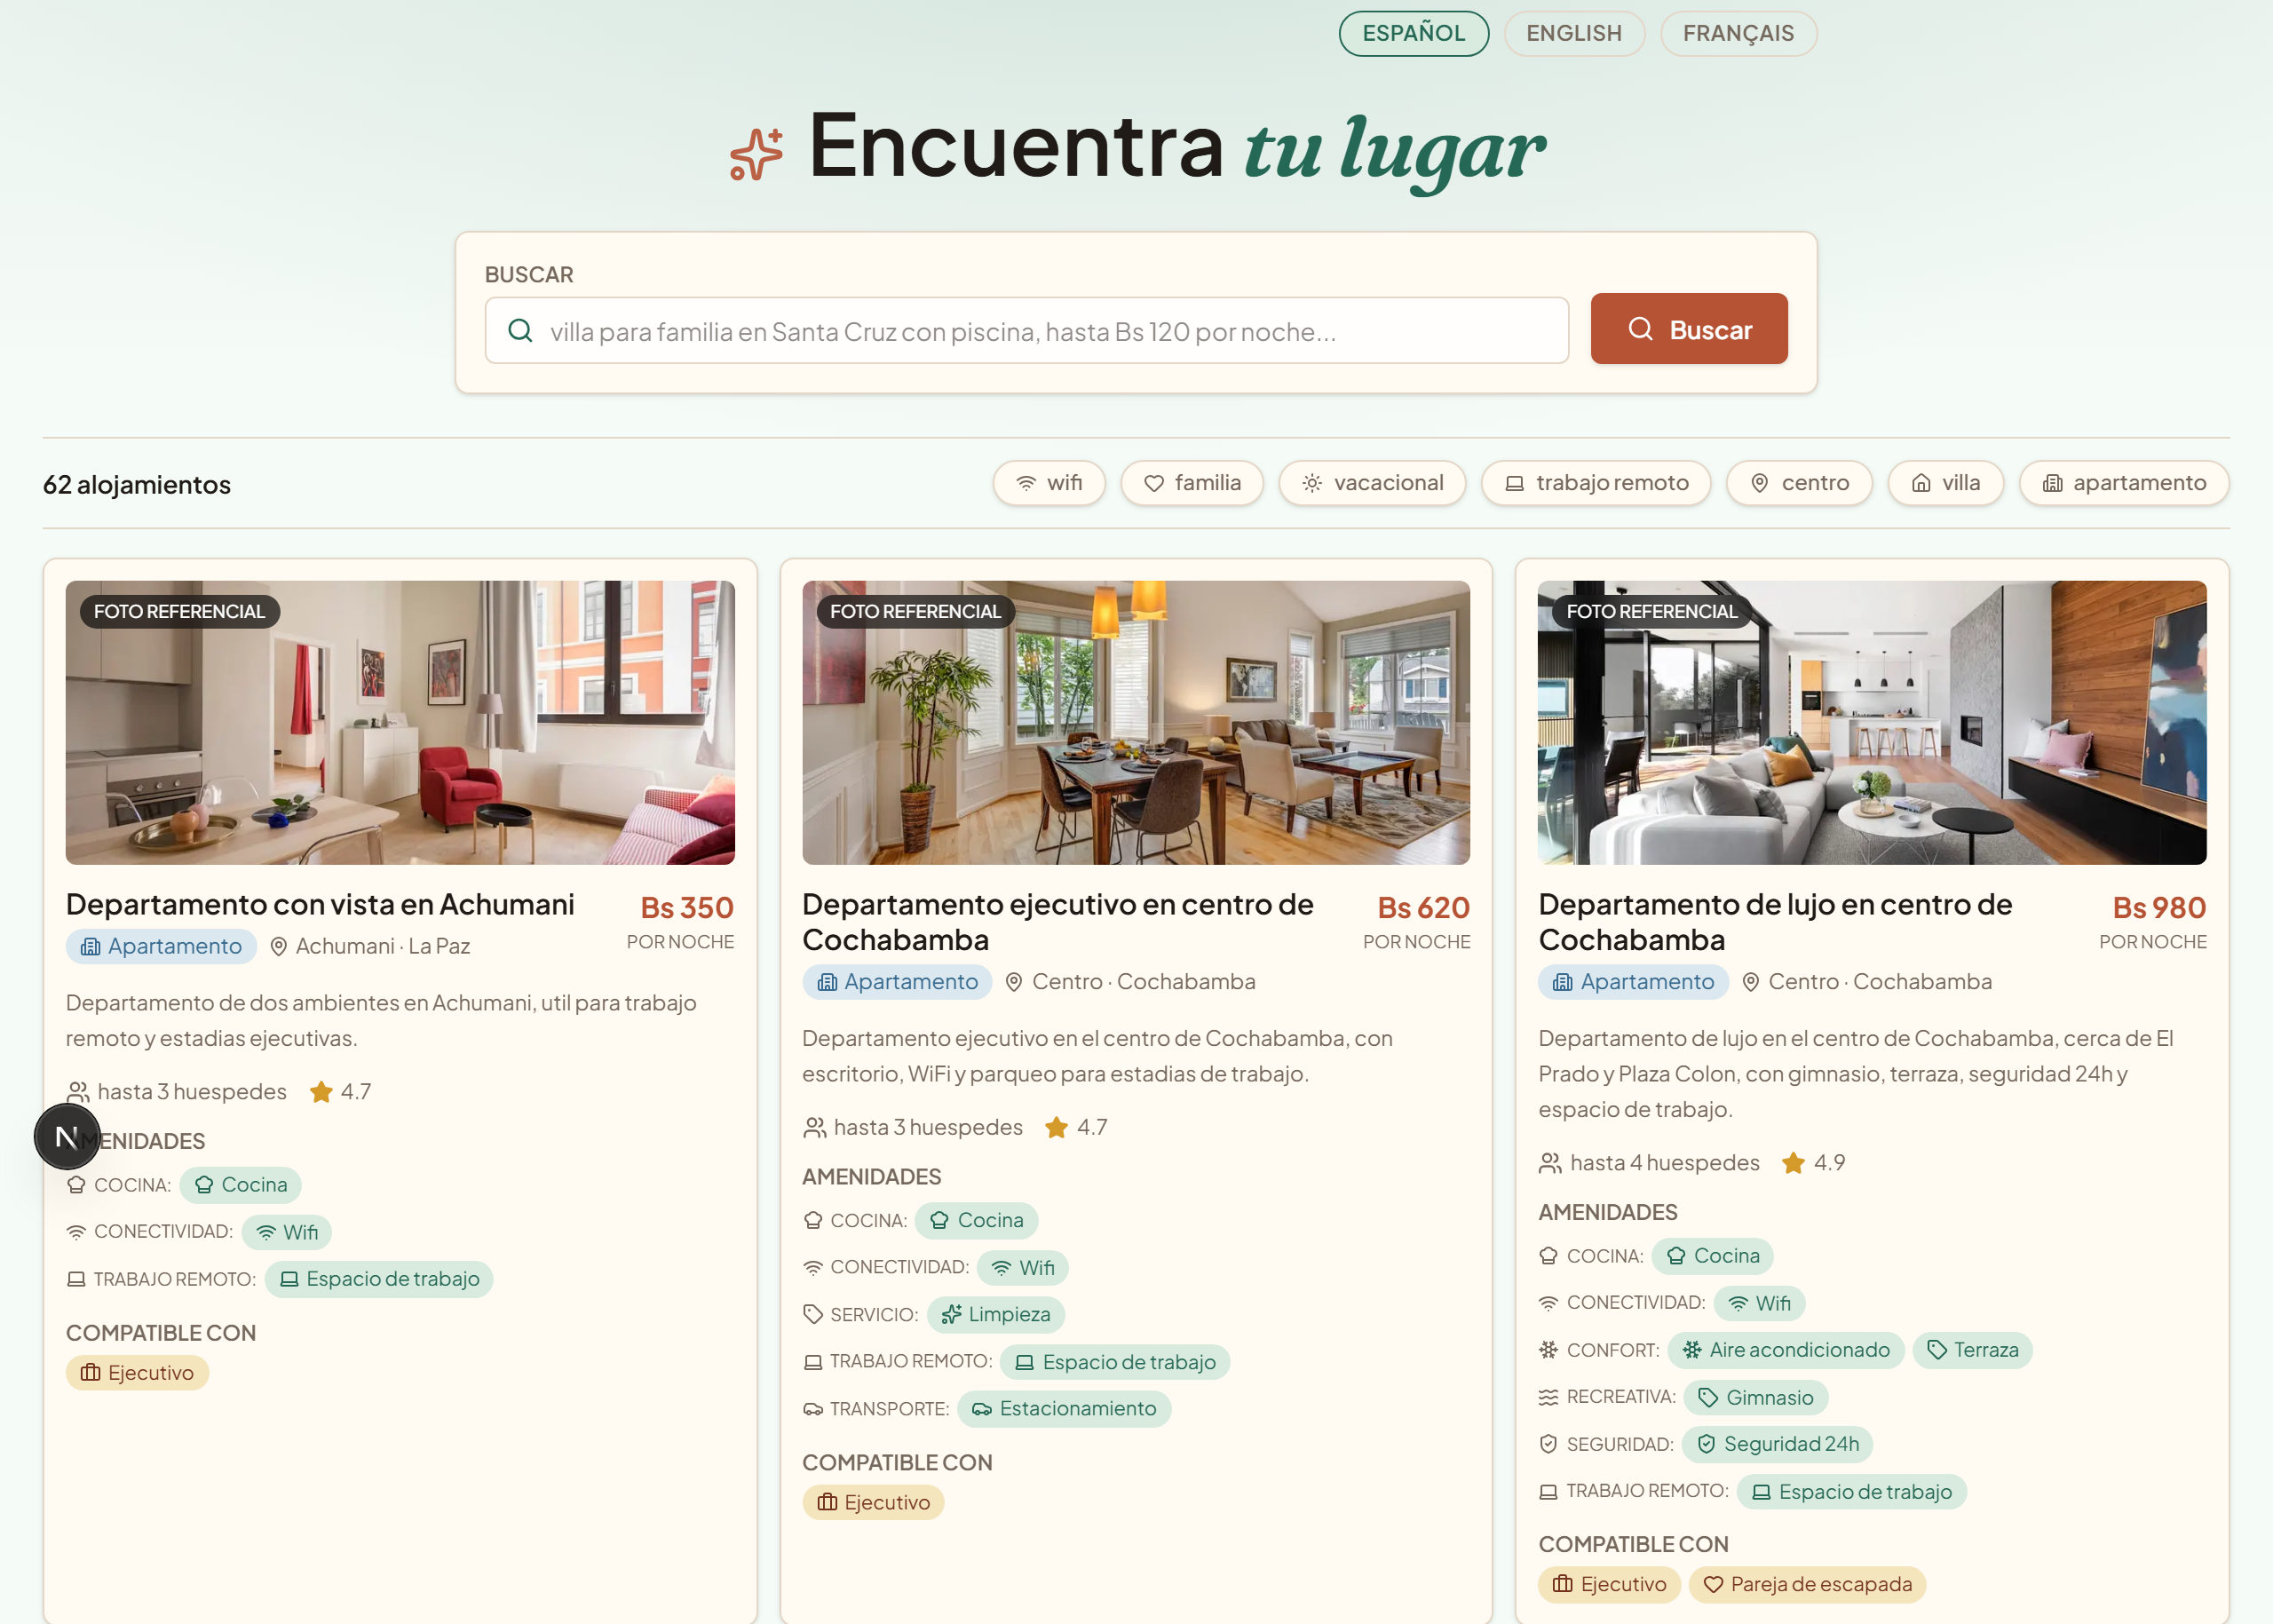
\includegraphics[width=0.9\textwidth]{images/ui_inicio_es.png}
\caption{Pantalla principal del buscador semántico en español.}
\label{fig:ui-es}
\end{figure}

\begin{figure}[H]
\centering

\includegraphics[width=0.9\textwidth]{images/ui_inicio_en.png}
\caption{Pantalla principal del buscador semántico en inglés sobre el mismo dataset OWL.}
\label{fig:ui-en}
\end{figure}

\begin{figure}[H]
\centering

\includegraphics[width=0.9\textwidth]{images/ui_inicio_fr.png}
\caption{Pantalla principal del buscador semántico en francés sobre el mismo dataset OWL.}
\label{fig:ui-fr}
\end{figure}

\begin{figure}[H]
\centering
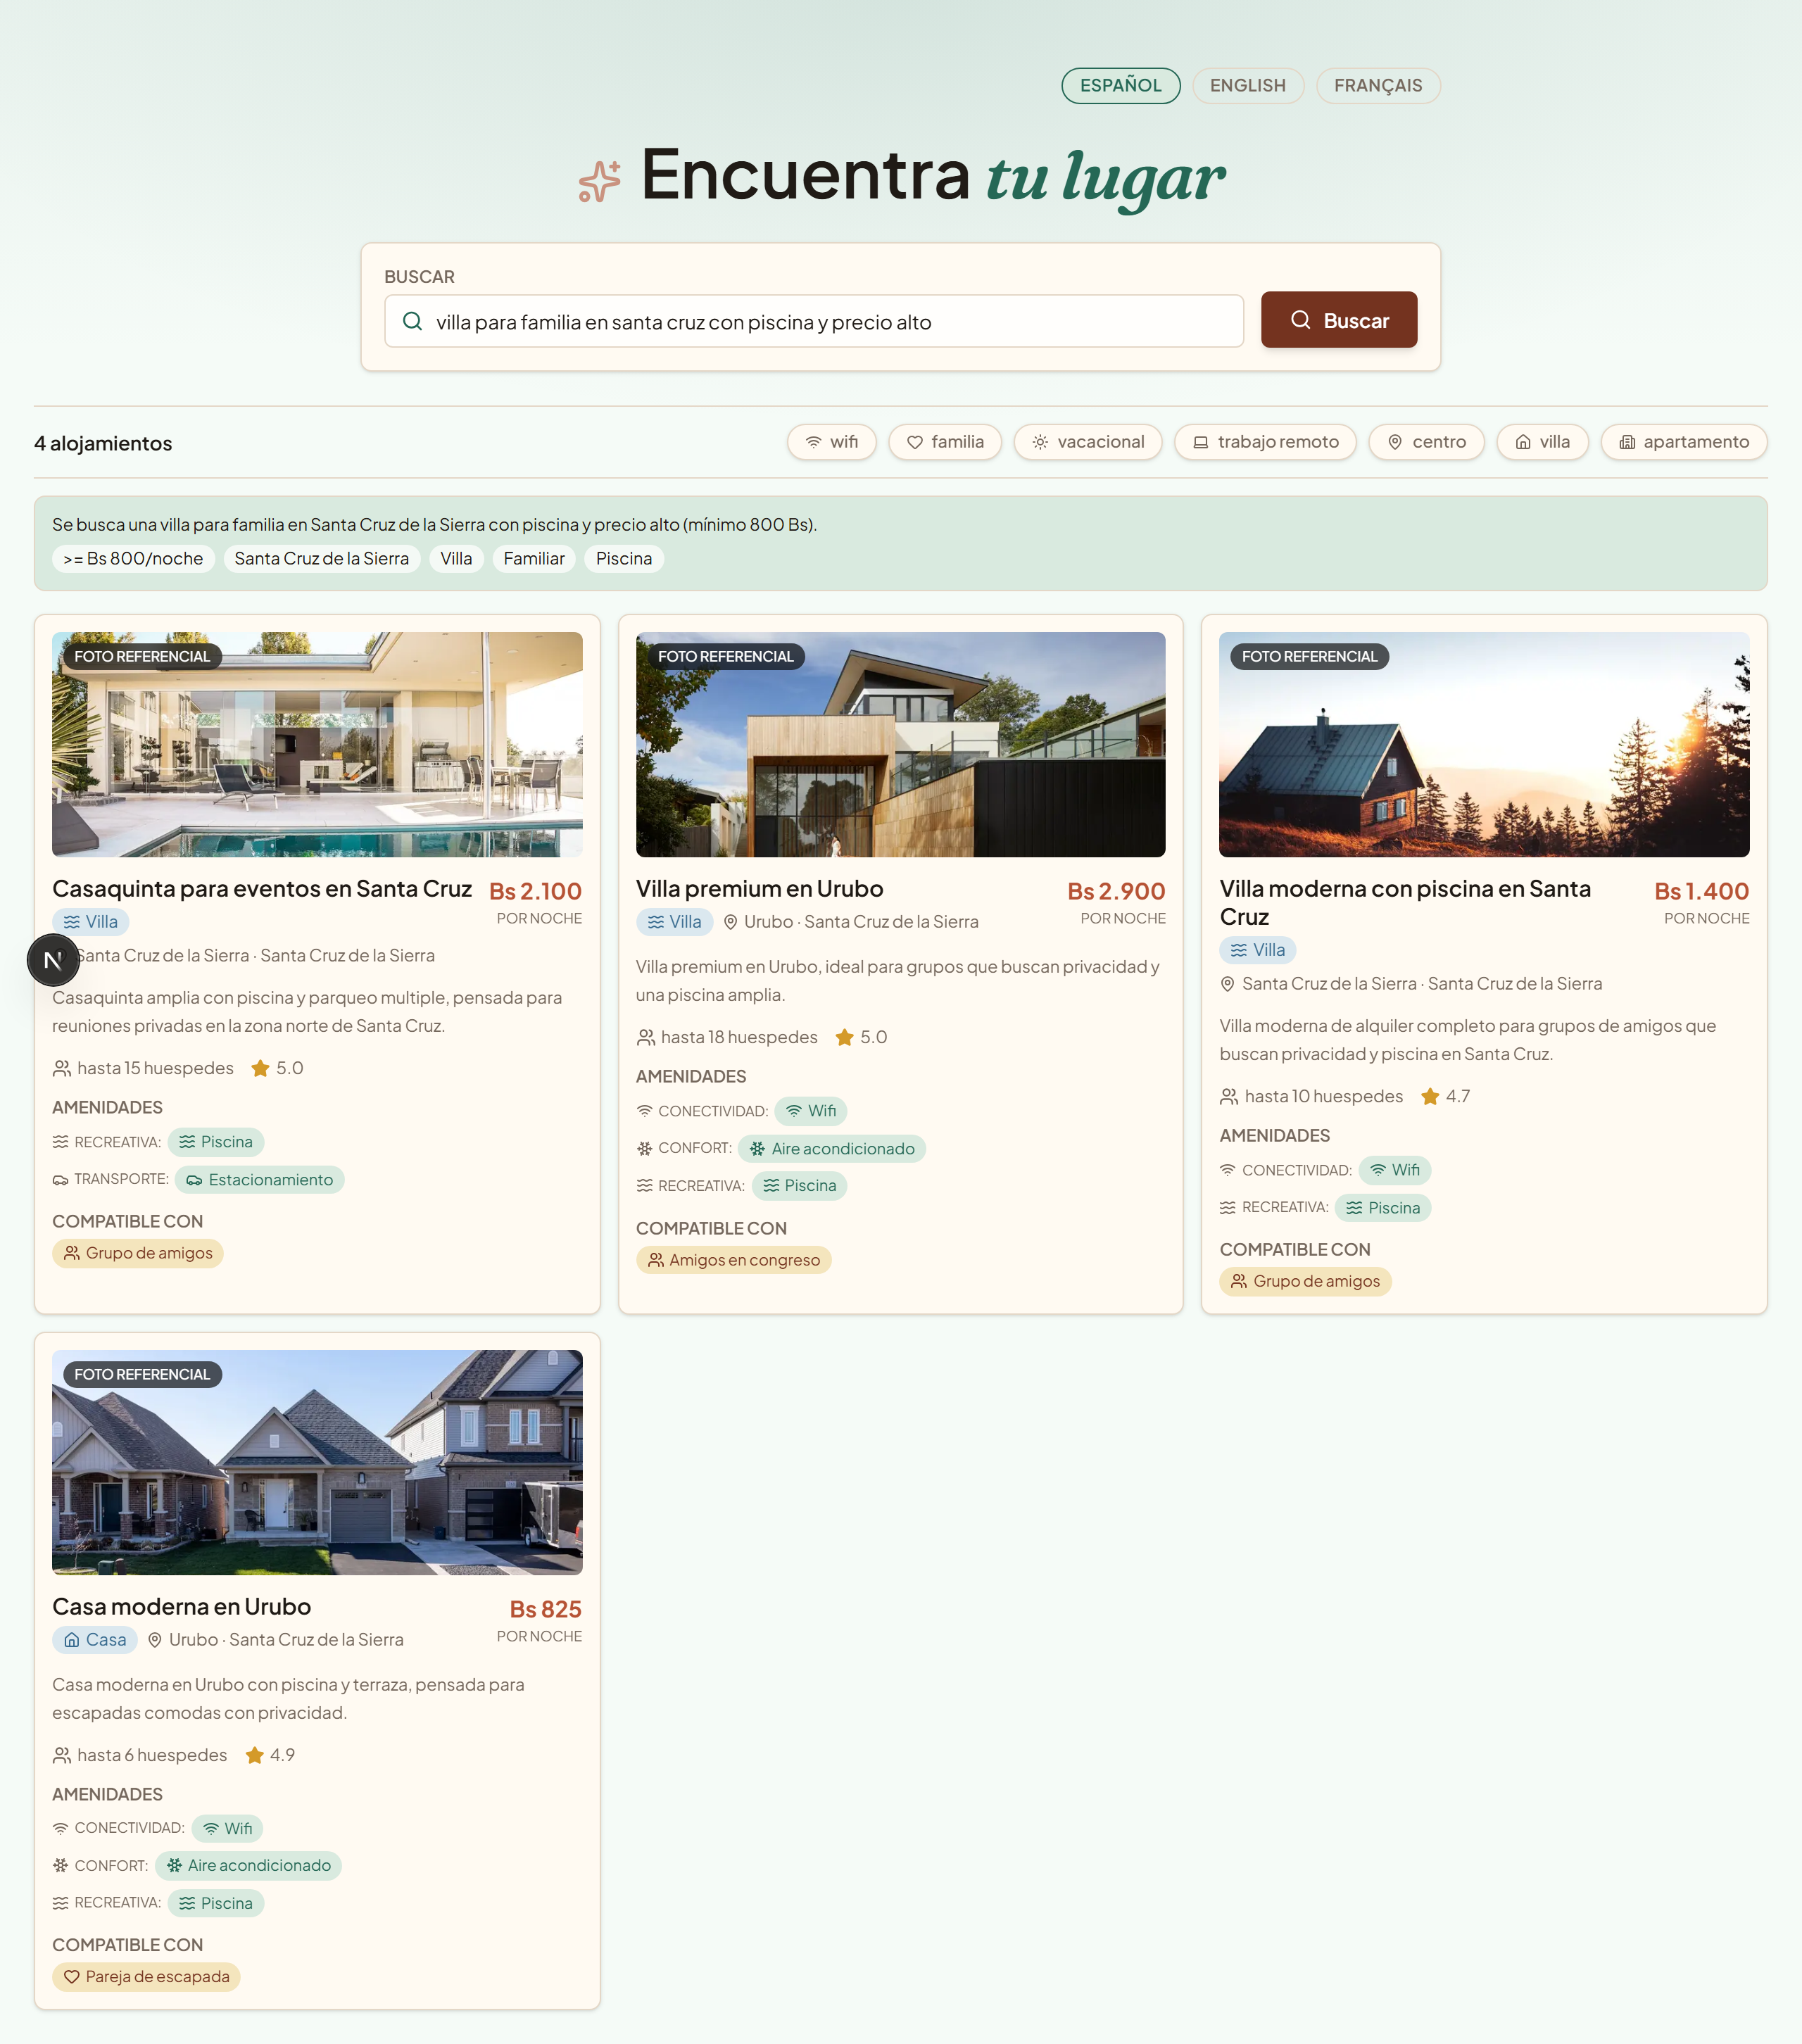
\includegraphics[width=0.9\textwidth]{images/ui_busqueda_compleja_es_1.png}
\caption{Resultado de una búsqueda compleja en español orientada a villas familiares en Santa Cruz con piscina y sesgo de precio alto.}
\label{fig:ui-es-compleja-1}
\end{figure}

\begin{figure}[H]
\centering
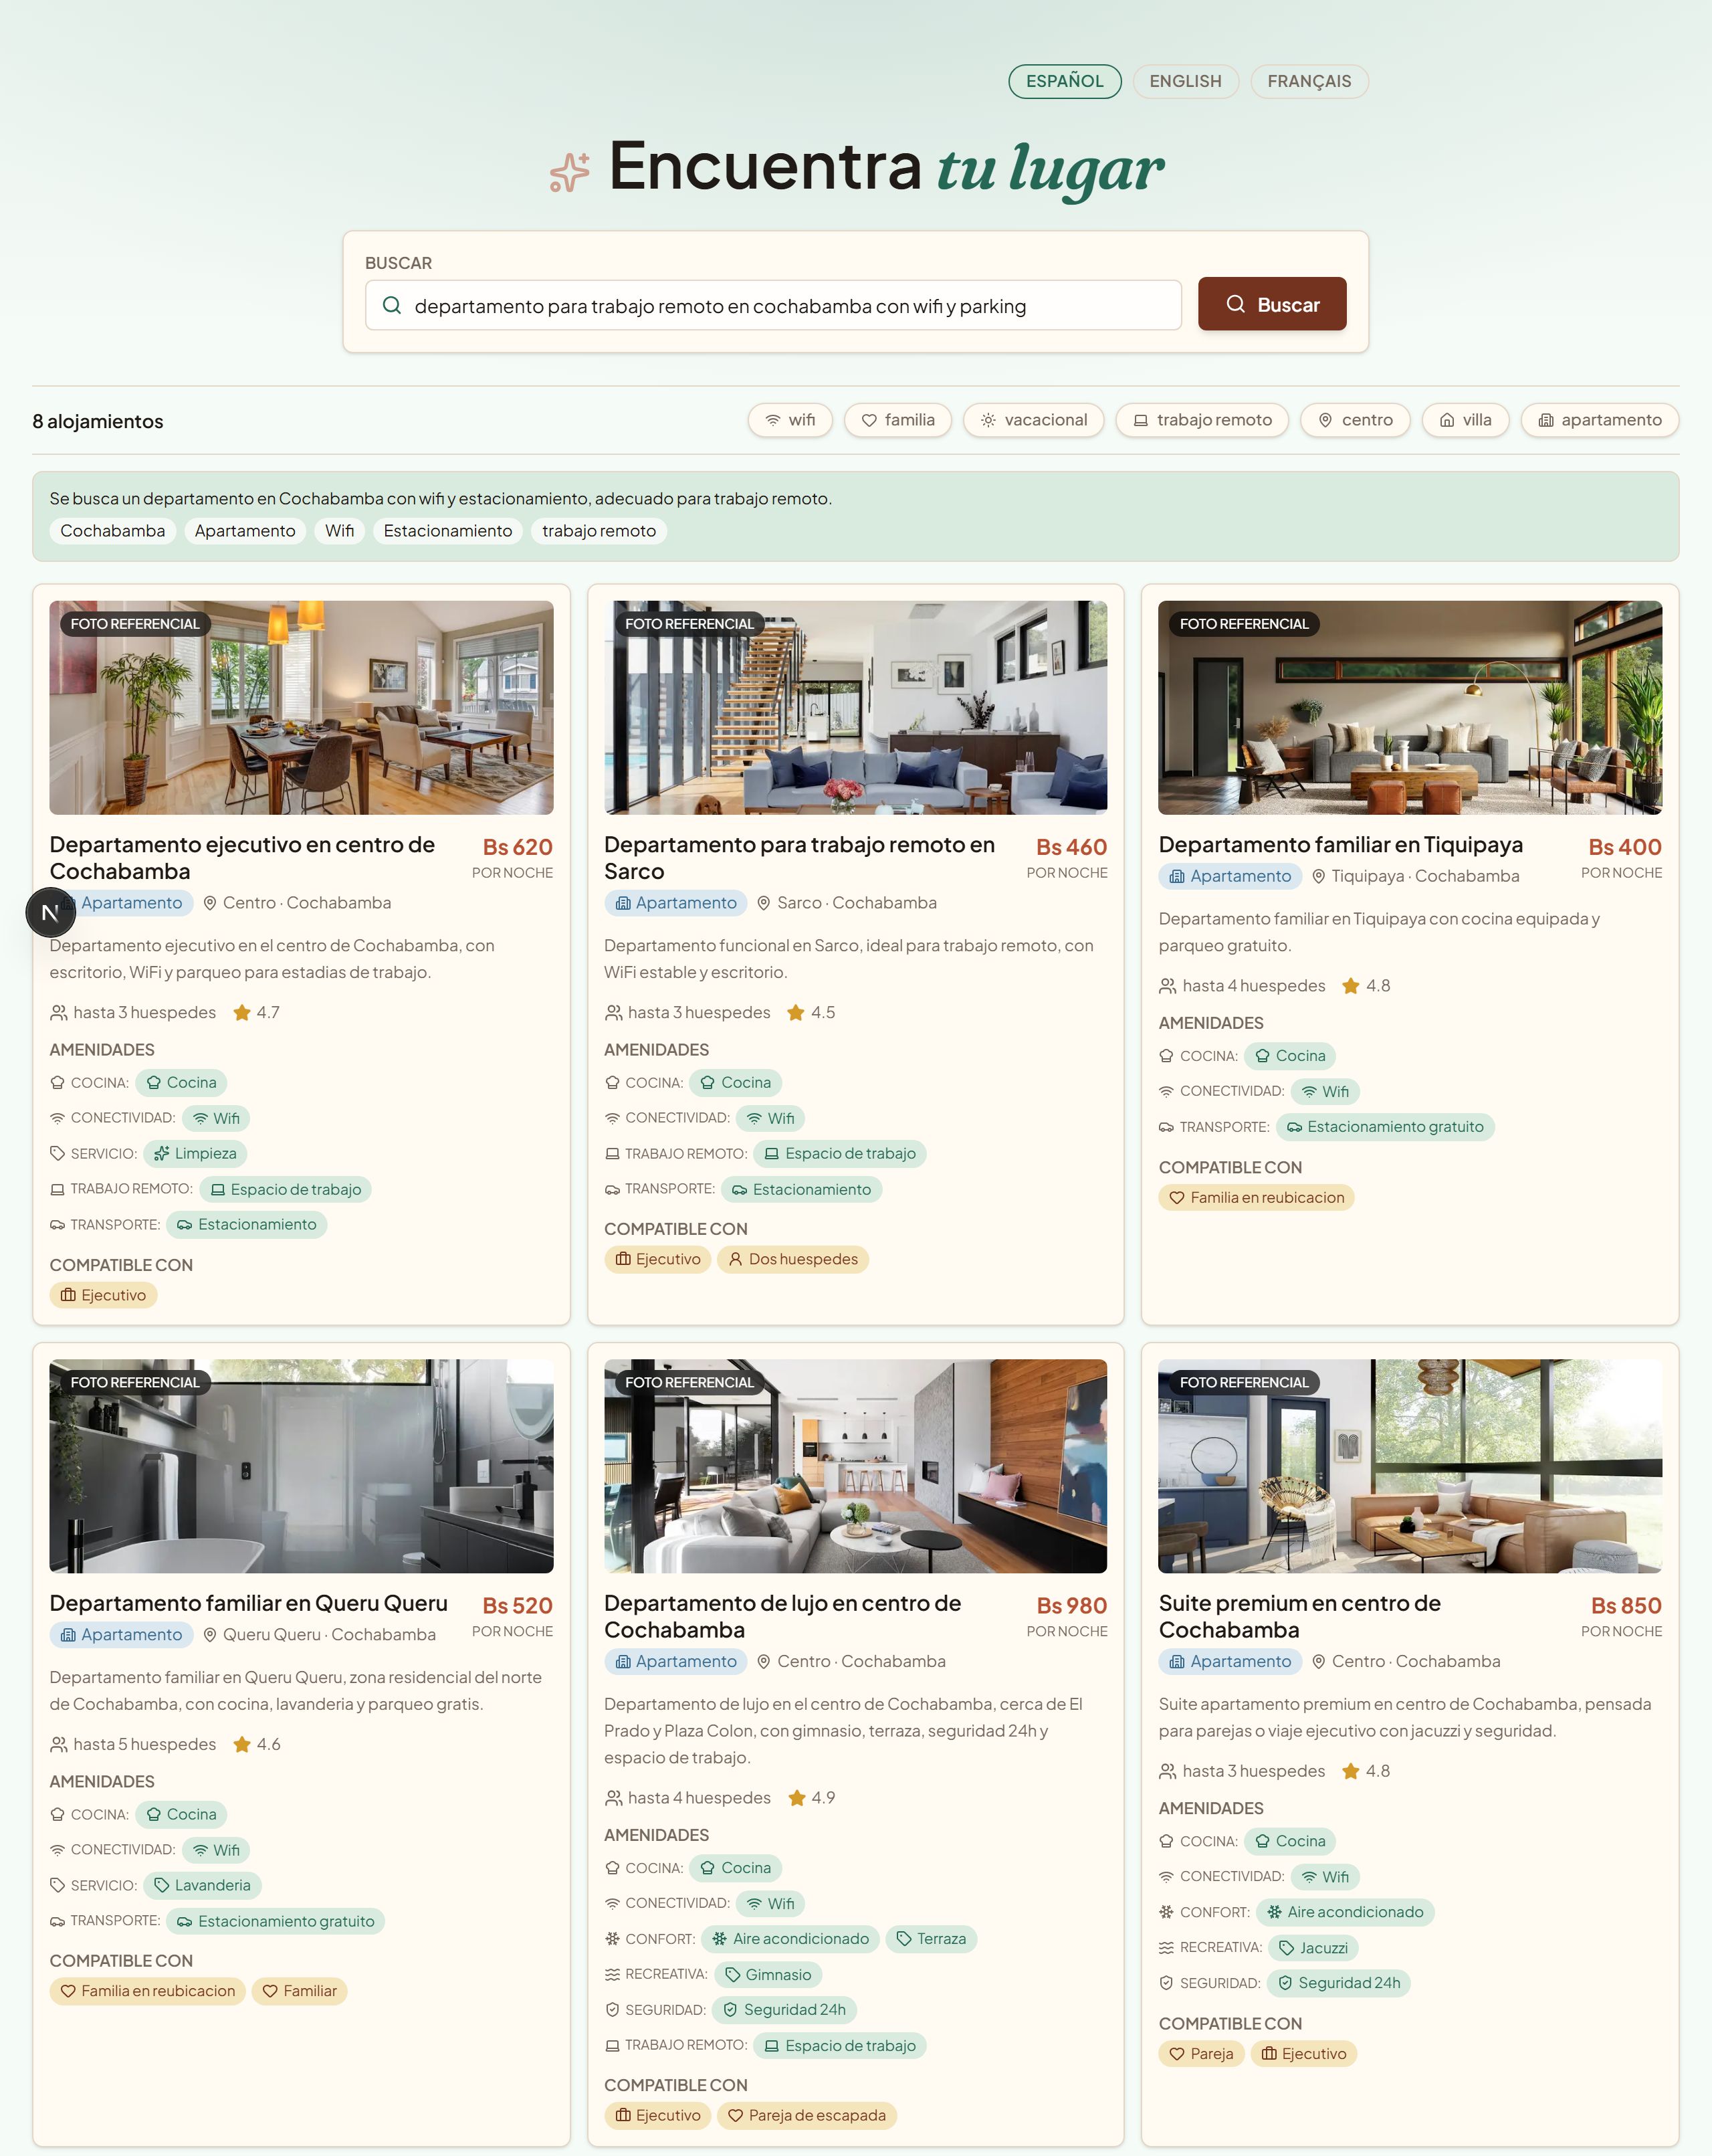
\includegraphics[width=0.9\textwidth]{images/ui_busqueda_compleja_es_2.png}
\caption{Resultado de una búsqueda compleja en español orientada a trabajo remoto en Cochabamba con Wi-Fi y estacionamiento.}
\label{fig:ui-es-compleja-2}
\end{figure}

\begin{figure}[H]
\centering
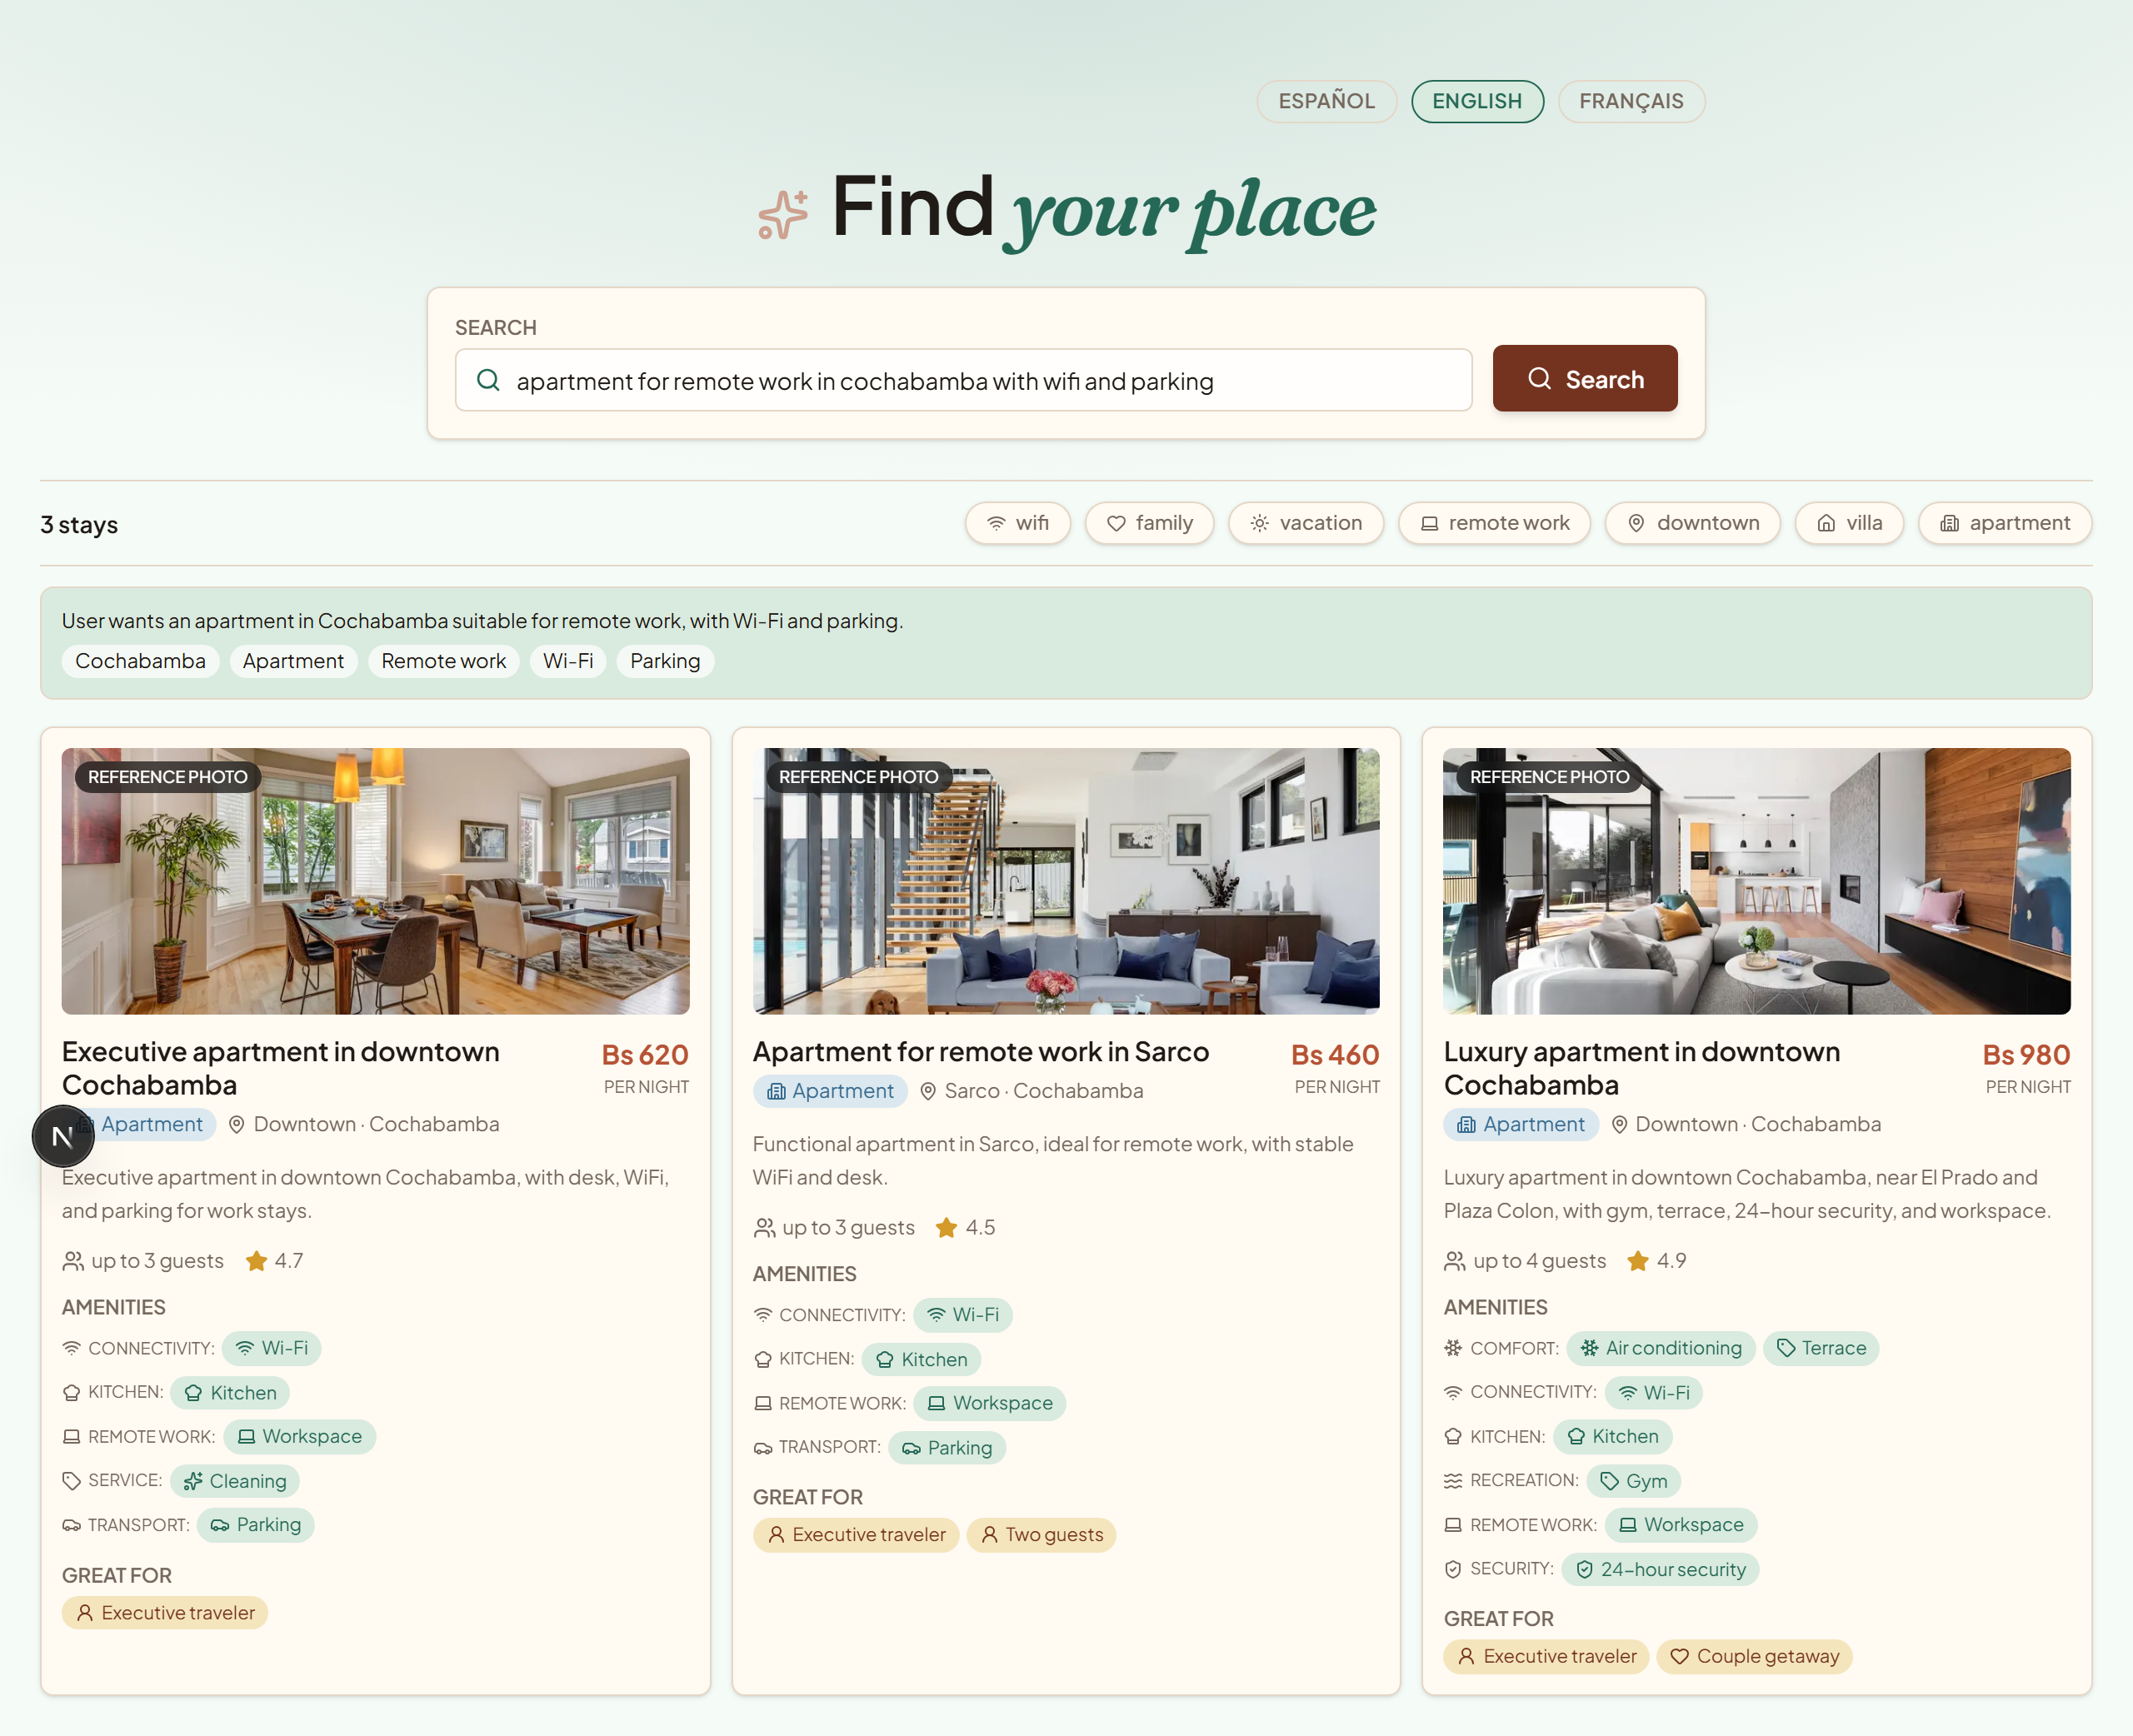
\includegraphics[width=0.9\textwidth]{images/ui_busqueda_compleja_en_1.png}
\caption{Resultado de la misma intención de búsqueda compleja en inglés, evidenciando recuperación semántica multilingüe.}
\label{fig:ui-en-compleja-1}
\end{figure}

\subsection{Valor técnico del prototipo}

La principal aportación técnica del sistema es demostrar que una ontología OWL puede ser
el centro operativo de un prototipo moderno de búsqueda, y no solo un modelo teórico.
La solución integra representación formal, consulta semántica, enriquecimiento con
Linked Data, multilingüidad real y una interfaz web usable. En consecuencia, el
proyecto cumple con el objetivo de aplicar investigación de Web Semántica en un
artefacto de software funcional, defendible y alineado con el enunciado de la práctica.
